\chapter{Project Development}
In this chapter, I will introduce how the project is developed,
the development tools and computational resources that I use for 
development.

This project tries to implement the two state-of-the-art models and 
expand their scope of application from datasets to arbitrary drawing.
Therefore, the whole project consists of two parts, training the deep 
learning models and building GUI to show the capability of the models.
Since training deep learning networks requires high computation power 
especially Graphics Processing Units(GPUs), which is not available to 
my laptop, so the plan is to train the models on Google Colab with 
free a GPU to use and then download the models and build a web app locally.

\section{Computational Resources}
Colaboratory brought by Google, often refered as Google Colab, is a 
free online interactive environment as the form of a jupyter notebook,
where we can write our python code and execute like our local jupyter 
notebook, furthermore, Google Colab has already configured most of the 
libraries for data science and machine learning, and it also provides 
a free GPU for us to use(K80, T4, P4, P100 will be allocated randomly).
However, it does have some problems, for example, sessions can get 
disconnected and accounts can be banned for long time continuously 
using the GPU. So my solution is to save the model checkpoints after 
certain epochs of training, since Colab allows users to mount their google drive, 
I set the checkpoints saving directory in google drive so that I can 
continue training when I get disconnected.
Despite these inconveniences, this is the best solution 
I can think of. 

\section{Deep Learning Framework}
The deep learning framework I choose for this project is PyTorch from Facebook. 
Pytorch offers tensor computation with strong GPU acceleration and deep neural 
networks built on a tape-based autograd system and it has become 
more and more popular in academia recently. Pytorch is friendly to tyros for 
you can easily understand what the code is doing and use the predefined 
frequently used layers such as convolution layers, batch normalization layers, 
etc. Also, it allows researchers to build deep neural networks with complex 
architectures flexibly which is an advantage over popular frameworks like Keras.
In addition, unlike Tensorflow, Pytorch uses dynamic computation graph instead 
of static computation graph which is beneficial for tweaking and debugging. And 
the most important advantage of Pytorch over Tensorflow for me is that Pytorch 
has better documentation than Tensorflow, for example, you may found several 
functions doing the thing under different packages in Tensorflow documentation,
which is kind of chaos. For more information about Pytorch please visit 
\href{https://pytorch.org/}{https://pytorch.org/}.

\section{Graphical User Interface}
I decided to use a web page as the graphical user interface(GUI) for my project.
Unlike C++ or $C\sharp$, python does not have powerful desktop application GUI 
frameworks, however, 
web development tools like Flask and Django for python can easily integrate the Pytorch 
library and can also make use of the front-end technology to make decent-looking 
GUI. When the user performs an action on the GUI, the front-end will send a request to 
the back-end, and the Flask framework will handle the request and ask Pytorch model to 
do the image translation if necessary. 

The front-end is basically developed with HTML, 
CSS, JavaScript, and libraries such as Bootstrap and Font Awesome.
In terms of back-end, I chose is Flask, which is a lightweight WSGI web application 
framework for python. Flask projects start with quick and easy setup but can scale 
up to complex applications, it also wraps Jinja2 which is a full-featured template 
engine that allows developers to integrate with front-end. 

The web app including 4 pages including a home page, an about page, two pages demonstrating
the capability of the model for translating segmentation maps in the dataset and arbitrary 
drawing semantic label maps respectively. 

\begin{figure}[H]
    \begin{center}
    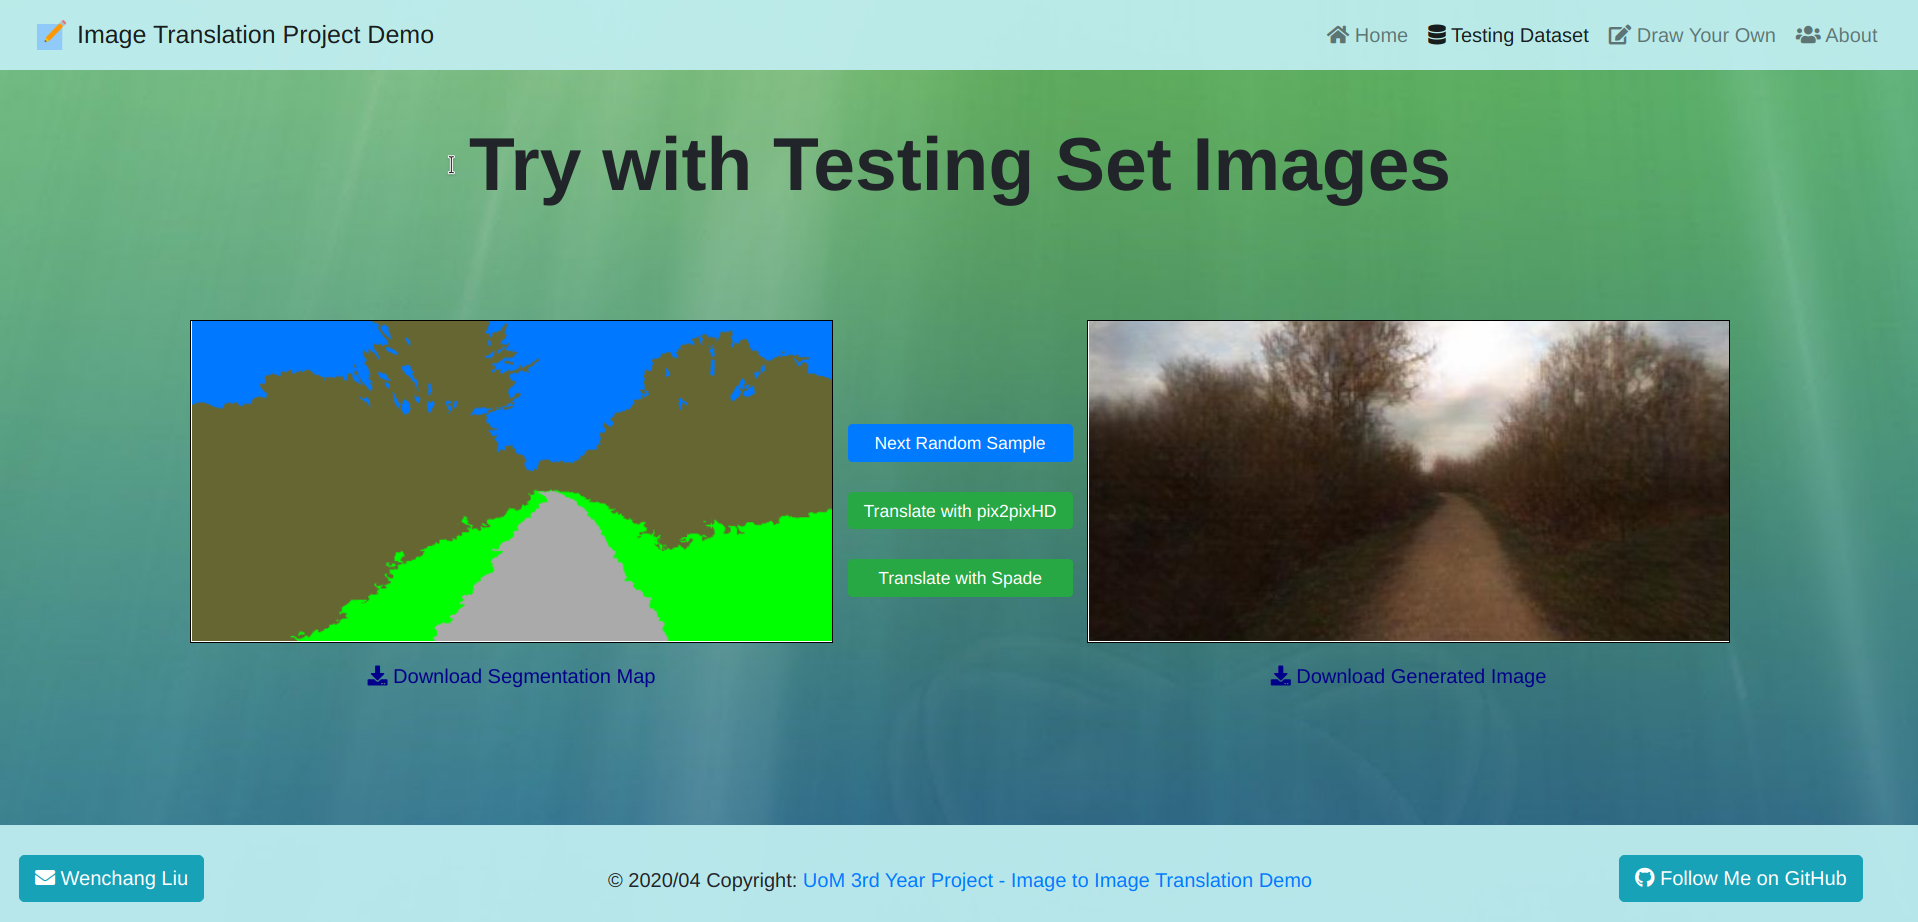
\includegraphics[width=14cm]{figures/GUI-testset}
    \end{center}
    \caption{Screenshot of the web page that allow users to try segmentation maps from the test dataset}
    \label{fig:GUI-testset}
\end{figure}

\begin{figure}[H]
    \begin{center}
    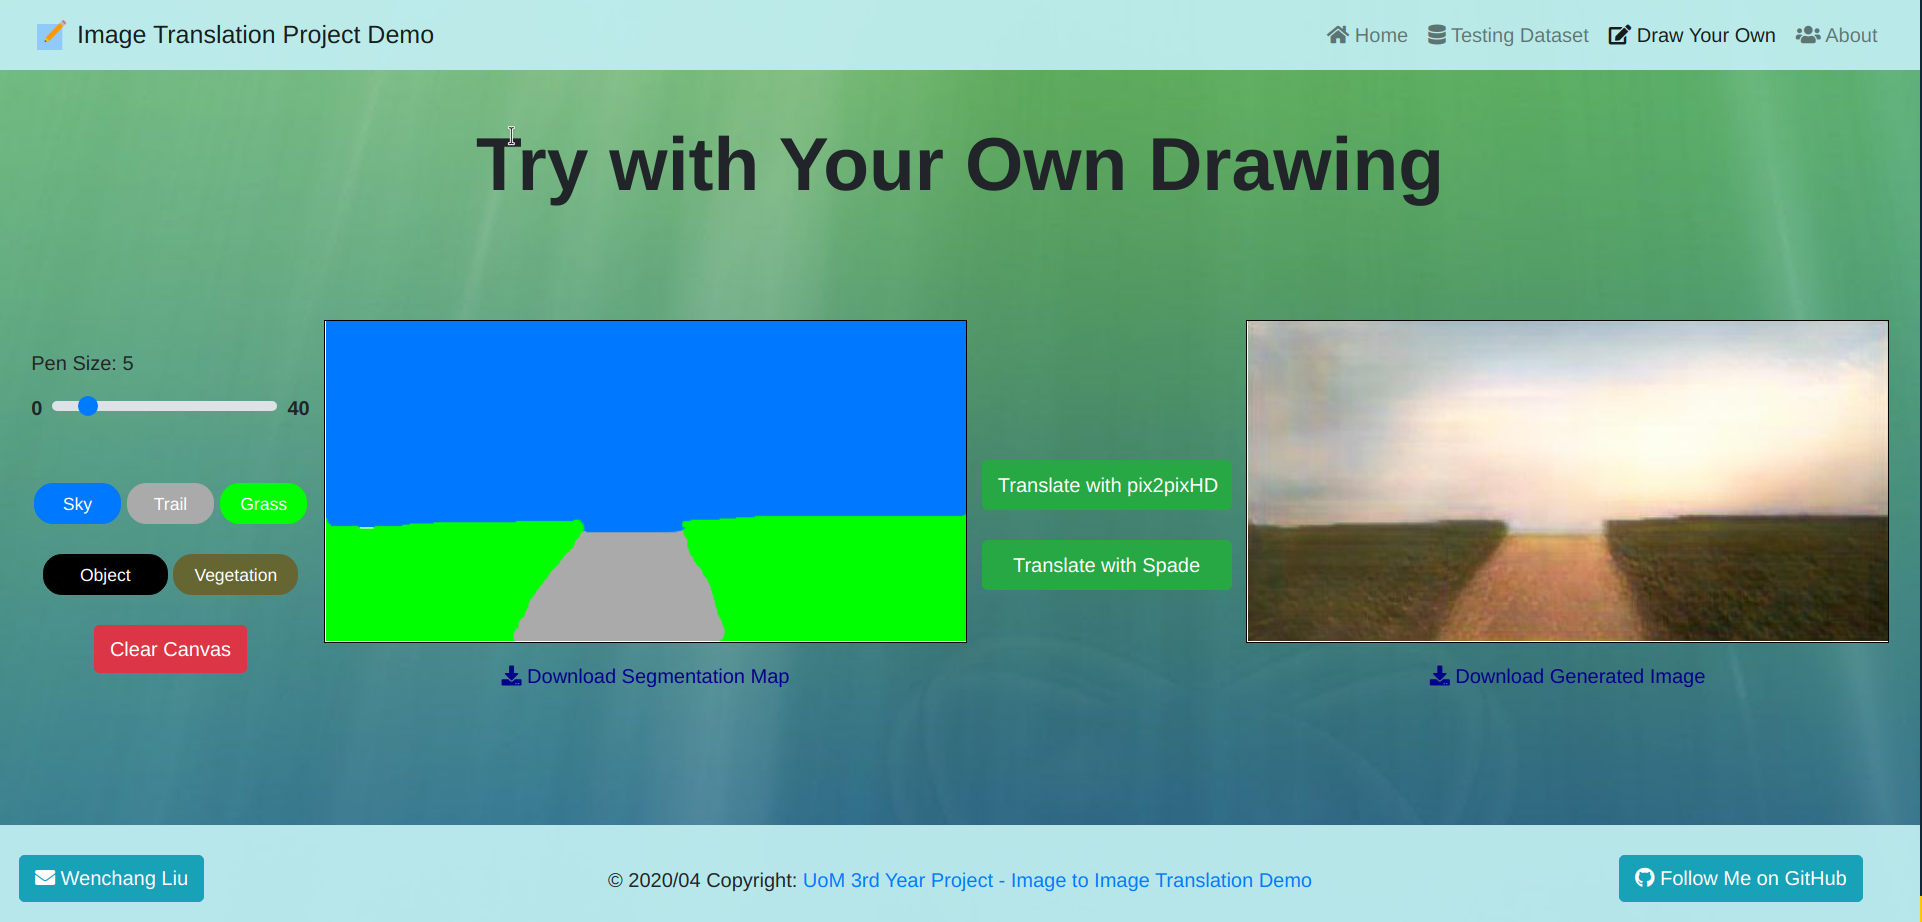
\includegraphics[width=14cm]{figures/GUI-draw}
    \end{center}
    \caption{Screenshot of the web page that allow users to try segmentation maps drawn by themselves}
    \label{fig:GUI-draw}
\end{figure}

The web app offers functionalities including getting next random sample segmentation map from 
the test dataset, simple drawing tool for users to draw their own style of segmentation map, 
downloading segmentation maps or generated photorealistic images, and translating the segmentation
map into photorealistic with both pix2pixHD and SPADE model.



% Local Variables: 
% mode: latex
% TeX-master: "report"
% End: 
